\documentclass[12pt,a4paper]{article}

\usepackage[T1]{fontenc}
\usepackage[french]{babel}
\usepackage[a4paper,margin=2cm]{geometry}
\usepackage{graphicx}
\usepackage{tikz}
\usepackage{array}
\usepackage{setspace}
\usepackage{xcolor}
\usepackage{fancyhdr}
\usepackage{lastpage} 
\usepackage[hidelinks]{hyperref}
\usepackage{tocloft}
\usepackage{etoolbox}

% Nom de la table des matières
\renewcommand{\contentsname}{Table des matières}

% Numérotation des sections en chiffres romains
\renewcommand{\thesection}{\Roman{section}-}

% Afficher les sous-sections dans la table
\setcounter{tocdepth}{2}

% Style de la table des matières
\renewcommand{\cftsecfont}{\bfseries}
\renewcommand{\cftsecpagefont}{\bfseries}

\pagestyle{fancy}

\fancyhf{}

\fancyfoot[R]{\small Page \thepage\ sur \pageref{LastPage}}

\renewcommand{\headrulewidth}{0pt}
\renewcommand{\footrulewidth}{0pt}
%%%%%%%%%%%%%%%%%%%%%%%%%%%%%%%%%%%%%%%%%%%%%%%%%%%%%%
% Chaque grande section commence sur une nouvelle page
%%%%%%%%%%%%%%%%%%%%%%%%%%%%%%%%%%%%%%%%%%%%%%%%%%%%%%

\pretocmd{\section}{\clearpage}{}{}

\begin{document}

\begin{center}

{\small\textbf{Ecole des Hautes Etudes des Sciences et Techniques de l'Ingénierie et du Management}}

\vspace{1cm}


%================ LOGOS ==================

\begin{minipage}{0.45\textwidth}
\centering

%------------------ Logo Ministère ------------------
\hspace{-5cm} 
\includegraphics[width=11 cm]{"logo_hestim.png.png"}

\end{minipage}
\hfill
\begin{minipage}{0.45\textwidth}
\centering

%------------------ Logo HESTIM ------------------
\hspace{-1cm}
\includegraphics[width=5cm]{"logo_mefb.jpg.jpg"}

\end{minipage}


\vspace{1cm}

{\bfseries Pôle ingénierie informatique et intelligence artificielle}

\vspace{1.5cm}


%%%%%%%%%%%%%%%%%%%%%%%%%%%%%%%%%%%%%%%%%%%%%%%%%%%%%%
% Bandeau professionnel du titre
%%%%%%%%%%%%%%%%%%%%%%%%%%%%%%%%%%%%%%%%%%%%%%%%%%%%%%

\begin{tikzpicture}

% Barre supérieure décorative
\draw[
green!50!black,
line width=3pt
]
(-6,2.25)--(6,2.25);


% Rectangle principal
\node[
draw=green!50!black,
line width=1.2pt,
rounded corners=8pt,
minimum width=12cm,
minimum height=4.5cm,
fill=white,
inner sep=12pt
]
{

\begin{minipage}{10.5cm}
\centering

{\Large\bfseries\color{green!50!black}
RAPPORT DE STAGE}

\vspace{0.4cm}

\rule{10cm}{0.5pt}

\vspace{0.4cm}

{\large\bfseries
MINISTÈRE DE L'ÉCONOMIE,}\\[0.15cm]

{\large\bfseries
DES FINANCES ET DU BUDGET}\\[0.15cm]

{\large\bfseries
DE LA RÉPUBLIQUE DE GUINÉE}

\vspace{0.45cm}

{\small
Stage réalisé dans le cadre de la formation\\
Cycle ingénieur en Informatique et Intelligence Artificielle
}

\end{minipage}

};

\end{tikzpicture}


\vspace{2cm}

\end{center}


\begin{flushleft}

\textbf{Réalisé par :} BALDE ABDOURAHAMANE DIOGO

\vspace{0.4cm}

\textbf{Encadrante :} MADAME MESKINI FATIMA ZAHRA

\vspace{0.4cm}

\textbf{Tuteur de stage :} MONSIEUR DIOP OUMAR
\vspace{0.4cm}

\textbf{Classe :} 1\textsuperscript{ère} année cycle ingénieur en informatique et intelligence artificielle.

\end{flushleft}


\vfill


\begin{flushleft}
Année scolaire 2025--2026
\end{flushleft}


\newpage

\begin{center}
{\Large\bfseries REMERCIEMENTS}
\end{center}

\vspace{1cm}

Je tiens à exprimer ma profonde gratitude au \textbf{MINISTÈRE DE L’ECONOMIE, DES FINANCES ET DU BUDGET DE LA RÉPUBLIQUE DE GUINÉE} et particulièrement à Monsieur Abdoulaye TOURE et à Madame KOUROUMA Emilie pour m'avoir offert l'opportunité enrichissante de réaliser mon stage au sein de la Direction Nationale des Systèmes Informatiques dudit Ministère.

\vspace{0.4cm}

Ce fut une expérience particulièrement enrichissante, tant sur le plan professionnel que personnel. Intégrer une structure d’une telle envergure m’a permis de découvrir un environnement de travail dynamique, rigoureux et exigeant, au cœur de l’un des secteurs les plus stratégiques du pays.

\vspace{0.4cm}

Je remercie également l’ensemble du personnel de la Direction pour leur accueil chaleureux, leur disponibilité et leur soutien constant. Leur encadrement m’a permis d’acquérir de nouvelles compétences techniques et pratiques, tout en développant un esprit de collaboration et de discipline professionnelle.

\vspace{0.4cm}

J’exprime toute ma gratitude à mon maître de stage ainsi qu’à l’ensemble de mes tuteurs, pour leur accompagnement, leurs conseils avisés et leur patience, qui ont grandement contribué à la réussite de cette expérience, sans oublier mon encadrante de stage \textbf{Madame MESKINI Fatima Zahra}, pour son suivi attentif et ses orientations constructives.

\vspace{0.4cm}

Je tiens également à remercier l’ensemble du corps professoral de \textbf{HESTIM}, pour leur encadrement et leur appui tout au long de mon parcours académique. Leur disponibilité et leurs encouragements m’ont permis de mieux tirer profit de ce stage et d’en faire une expérience pleinement enrichissante.

\vspace{0.4cm}

Cette immersion restera pour moi une étape déterminante dans mon parcours académique et professionnel, et je suis convaincu que les acquis de ce stage me serviront de base solide pour mes projets futurs.

\newpage

%%%%%%%%%%%%%%%%%%%%%%%%%%%%%%%%%%%%%%%%%%%%%%%%%%%%%%
% TABLE DES MATIÈRES
%%%%%%%%%%%%%%%%%%%%%%%%%%%%%%%%%%%%%%%%%%%%%%%%%%%%%%

\tableofcontents
%%%%%%%%%%%%%%%%%%%%%%%%%%%%%%%%%%%%%%%%%%%%%%%%%%%%%%
% LISTE DES SIGLES ET ABRÉVIATIONS
%%%%%%%%%%%%%%%%%%%%%%%%%%%%%%%%%%%%%%%%%%%%%%%%%%%%%%

\clearpage

\begin{center}
{\Large\bfseries LISTE DES SIGLES ET ABRÉVIATIONS}
\end{center}

\vspace{1cm}

\begin{center}
\renewcommand{\arraystretch}{2}
\begin{tabular}{|p{3cm}|p{11cm}|}
\hline
\textbf{MEFB} & Ministère de l'Économie, des Finances et du Budget \\ \hline
\textbf{DNSI} & Direction Nationale des Systèmes Informatiques \\ \hline
\end{tabular}
\end{center}

%%%%%%%%%%%%%%%%%%%%%%%%%%%%%%%%%%%%%%%%%%%%%%%%%%%%%%
% LISTE DES FIGURES
%%%%%%%%%%%%%%%%%%%%%%%%%%%%%%%%%%%%%%%%%%%%%%%%%%%%%%

\clearpage

\begin{center}
{\Large\bfseries LISTE DES FIGURES}
\end{center}

\vspace{1cm}

\begin{center}
\renewcommand{\arraystretch}{1.8}
\begin{tabular}{|p{10cm}|p{2.6cm}|p{1.8cm}|}
\hline
\textbf{Description} & \textbf{Figure} & \textbf{Page} \\ \hline

Diagramme de cas d'utilisation & Figure 1 & \pageref{fig:cas-utilisation} \\ \hline
Diagramme de classes du modèle de données & Figure 2 & \pageref{fig:classes} \\ \hline
Diagramme de séquence du parcours de validation & Figure 3 & \pageref{fig:sequence} \\ \hline
Diagramme d'état d'une demande de congé & Figure 4 & \pageref{fig:etat-demande} \\ \hline
Diagramme d'état d'une étape de validation & Figure 5 & \pageref{fig:etat-etape} \\ \hline

\end{tabular}
\end{center}

%%%%%%%%%%%%%%%%%%%%%%%%%%%%%%%%%%%%%%%%%%%%%%%%%%%%%%
% INTRODUCTION
%%%%%%%%%%%%%%%%%%%%%%%%%%%%%%%%%%%%%%%%%%%%%%%%%%%%%%

\section{INTRODUCTION}

Le stage est une étape très importante dans le parcours d’un étudiant, car il permet de mettre en pratique les connaissances apprises à l’école et de découvrir la réalité du monde professionnel. Il donne aussi l’occasion de mieux comprendre le fonctionnement d’une entreprise et d’apprendre de nouvelles compétences utiles pour l’avenir.
Dans ce cadre, j’ai eu la chance d’effectuer mon stage au MINSTERE DE L’ECONOMIE, DES FINANCES ET DU BUDGET(MEFB) plus précisément à la Direction Nationale des Systèmes Informatiques (DNSI) . C’est une structure de grande importance en Guinée, qui offre un environnement de travail sérieux et enrichissant dans le domaine informatique.
Ce stage m’a permis d’approfondir mes connaissances en informatique, d’apprendre de nouvelles méthodes de travail et de comprendre l’importance des systèmes informatiques au sein d’un ministère en charge de l’économie du pays. J’ai aussi beaucoup appris sur le plan humain, en développant des qualités comme la rigueur, le travail en équipe et la discipline.
Ce rapport présente le déroulement de mon stage. Il est organisé en plusieurs parties : la présentation de la structure d’accueil, la description de la DNSI et des missions que j’ai réalisées, puis une analyse des acquis et des difficultés rencontrées, avant de terminer par une conclusion et quelques recommandations


%%%%%%%%%%%%%%%%%%%%%%%%%%%%%%%%%%%%%%%%%%%%%%%%%%%%%%
% PRÉSENTATION DE L'ENTREPRISE
%%%%%%%%%%%%%%%%%%%%%%%%%%%%%%%%%%%%%%%%%%%%%%%%%%%%%%

\section{PRÉSENTATION DU MINISTERE DE L'ECONOMIE, DES FINANCES ET DU BUDGET}

\subsection{Historique du MEFB}

Fondé dès l'accession de la Guinée à l'indépendance en 1958, le ministère a vu sa dénomination et l'étendue de ses compétences fluctuer au gré des réformes institutionnelles. C’est précisément le 30 avril 1959 qu'apparaît pour la première fois l'appellation explicite de Ministère des Finances, des Affaires Économiques et du Plan. Plus récemment, sous la transition dirigée par le Général Mamadi Doumbouya, les portefeuilles de l'Économie, des Finances et du Budget ont été regroupés pour optimiser l'action de l'État.

\subsection{Organisation (organigramme simplifié)}

L’appareil administratif du MEFB est structuré de manière hiérarchique pour assurer une exécution fluide des réformes publiques :Le Cabinet du Ministre : Composé du Secrétaire Général, du Chef de Cabinet, de conseillers sectoriels et de services d'appui directs.Les Directions Nationales et Générales : Notamment la Direction Générale du Budget (DGB), la Direction Générale des Impôts (DGI), la Direction Générale des Douanes (DGD), ainsi que les directions chargées du Trésor, de la Dette publique, et du Contrôle Financier.Organismes sous tutelle : Il exerce son contrôle sur plusieurs Établissements Publics Administratifs (EPA) et assure la tutelle financière des entreprises publiques.

\subsection{Missions principales du MEFB}

Conformément au cadre réglementaire en vigueur, le ministère est particulièrement investi des missions suivantes :Conception et arbitrage budgétaire : Coordonner la préparation, l'élaboration et l'exécution des lois de finances et de la programmation budgétaire pluriannuelle.Mobilisation des ressources : Maximiser la collecte des recettes fiscales, douanières et non fiscales nécessaires au financement de l'État.Gestion de la dépense publique : Veiller à la transparence, à la régularité et à la qualification de la dépense publique.Politique monétaire et endettement : Négocier les financements extérieurs, encadrer les partenariats public-privé (PPP) et piloter la politique d'endettement pour maintenir les équilibres macroéconomiques.

\subsection{Vision du MEFB}

La vision à long terme du MEFB s'aligne sur les orientations nationales de l'Étude Prospective « Guinée, Vision 2040 » et le déploiement du programme Simandou 2040. Les priorités stratégiques du ministère se fondent sur :La refondation de l'État : Instaurer une gestion dépersonnalisée, intègre et dépolitisée des institutions financières.La lutte contre la prévarication : Éradiquer la corruption, la fraude fiscale et le détournement des deniers publics par une transparence accrue (ex: déploiement du système SICOF).Le développement souverain : Transformer durablement les ressources naturelles du pays pour en faire le levier financier des générations futures, notamment à travers le Fonds Souverain de Guinée (FSG).

%%%%%%%%%%%%%%%%%%%%%%%%%%%%%%%%%%%%%%%%%%%%%%%%%%%%%%
% SERVICE D'ACCUEIL
%%%%%%%%%%%%%%%%%%%%%%%%%%%%%%%%%%%%%%%%%%%%%%%%%%%%%%

\section{PRÉSENTATION DE LA DIRECTION D'ACCUEIL}

\subsection{Description Générale}

La Direction Nationale des Systèmes Informatiques (DNSI) de Guinée conçoit, élabore et met en œuvre la politique informatique du Ministère du Budget et du Ministère de l'Économie, des Finances et du Budget.
La DNSI est un service central du département ministériel chargé de l'économie, des finances et du budget. Elle joue un rôle clé dans la modernisation de l'administration financière en intégrant les outils numériques dans la gestion publique.

\subsection{HISTORIQUE ET VISION}

La DNSI participe aux réformes de modernisation de l'État et s'appuie sur des cadres stratégiques tels que le plan PASANDAD (2016-2020). Sa vision vise à instaurer une administration publique digitalisée et performante pour optimiser la gestion budgétaire.

\subsection{Missions principales}

Conception : Élaborer la politique informatique globale des ministères partenaires.Mise en œuvre : Déployer les solutions et infrastructures technologiques nécessaires aux services financiers.Suivi : Assurer la maintenance, l'évolution et le contrôle des systèmes informatiques mis en place.

%%%%%%%%%%%%%%%%%%%%%%%%%%%%%%%%%%%%%%%%%%%%%%%%%%%%%%
% DÉROULEMENT DU STAGE
%%%%%%%%%%%%%%%%%%%%%%%%%%%%%%%%%%%%%%%%%%%%%%%%%%%%%%

\section{DÉROULEMENT DU STAGE}

\subsection{Objectif du stage}

L’objectif principal de ce stage est de mettre en pratique les connaissances acquises au cours de ma formation et de les confronter aux réalités du monde professionnel. Ce stage constitue également une occasion de découvrir le fonctionnement d’une entreprise, de comprendre son organisation et ses méthodes de travail.

Il vise aussi à développer mes compétences techniques et professionnelles à travers la participation à des missions concrètes, tout en améliorant mon autonomie, ma capacité à travailler en équipe et ma capacité à résoudre des problèmes. Enfin, cette expérience me permet de mieux comprendre les exigences du milieu professionnel et de préciser progressivement mon projet professionnel.


\subsection{Intégration dans la DNSI}

Dès les premiers jours de mon stage au sein du Ministère de l’Économie, des Finances et du Budget, j’ai été accueilli et orienté afin de mieux comprendre l’organisation et le fonctionnement de l’institution. Cette première étape m’a permis de découvrir l’environnement professionnel dans lequel j’allais évoluer ainsi que les principales règles et consignes à respecter au sein de l’administration.

J’ai ensuite été accueilli au sein du service informatique, où j’ai fait la connaissance des différents membres de l’équipe et de mes encadreurs de stage. Une présentation du service m’a permis de mieux comprendre son organisation, ses missions et son rôle dans le fonctionnement quotidien du Ministère.

Le service informatique assure notamment la gestion et la maintenance des équipements informatiques, l’assistance technique aux différents services, ainsi que le suivi des infrastructures et des outils informatiques utilisés par les agents. Cette présentation m’a permis de comprendre l’importance du service informatique dans le bon fonctionnement des activités administratives du Ministère.

Au cours de cette première période, j’ai également pris connaissance des méthodes de travail, des procédures internes et des consignes de sécurité liées à l’utilisation des équipements et des ressources informatiques. L’accueil et les échanges avec les membres du service m’ont facilité mon intégration et m’ont permis de m’adapter progressivement à mon nouvel environnement de travail.

Cette phase d’intégration a constitué une étape importante de mon stage, car elle m’a permis de mieux comprendre le fonctionnement du service, de créer de bonnes relations professionnelles avec l’équipe et d’aborder les différentes missions qui m’ont été confiées dans de bonnes conditions.


\subsection{Missions et tâches réalisées}

La mission principale qui m'a été confiée durant ce stage consistait à concevoir et développer une application de gestion des congés pour le Ministère de l'Économie, des Finances et du Budget. Le processus en vigueur reposait jusque-là sur un circuit entièrement manuel~: une demande de congé rédigée sur papier devait être transmise physiquement au chef de service, puis au directeur, puis au chef de cabinet, avant qu'une attestation ne soit délivrée à l'agent. Ce fonctionnement rendait le suivi des demandes difficile et ne permettait aucune vérification fiable de l'authenticité des attestations délivrées. L'objectif de ma mission était de dématérialiser l'ensemble de ce processus tout en respectant fidèlement le circuit hiérarchique propre au ministère.

\subsubsection{Analyse de l'existant et choix d'architecture}

J'ai commencé par analyser en détail une solution libre de gestion des ressources humaines déjà utilisée dans d'autres contextes, frappe/hrms, afin d'en tirer les enseignements applicables au projet avant de me lancer dans le développement. Cette analyse m'a permis d'identifier les limites d'une approche généraliste pour ce besoin précis, notamment l'absence d'un circuit de validation à plusieurs niveaux et l'absence de tout mécanisme d'authentification des documents délivrés. Sur cette base, et en accord avec les orientations techniques du ministère, j'ai opté pour une réécriture complète de l'application avec Django et Django REST Framework côté serveur, React et TypeScript côté interface, et PostgreSQL pour le stockage des données.

\subsubsection{Conception du modèle de données et du circuit de validation}

J'ai modélisé les différents types de congés prévus par le cahier des charges (congé normal, congé de maternité, congé de maladie à courte et longue durée, congé de formation, congé exceptionnel), chacun avec ses propres règles de durée et ses propres justificatifs obligatoires, de manière paramétrable plutôt que codée en dur. J'ai ensuite conçu le cœur métier de l'application~: un circuit de validation hiérarchique dont le nombre d'étapes s'adapte automatiquement au rôle du demandeur. Un agent voit sa demande remonter successivement au chef de service, au directeur puis au chef de cabinet, tandis qu'un chef de service ou un directeur qui dépose lui-même une demande voit son propre niveau sauté dans le circuit.

\subsubsection{Diagrammes de conception}

Pour formaliser cette conception avant de la développer, j'ai produit les diagrammes UML suivants.

\begin{figure}[htbp]
    \centering
    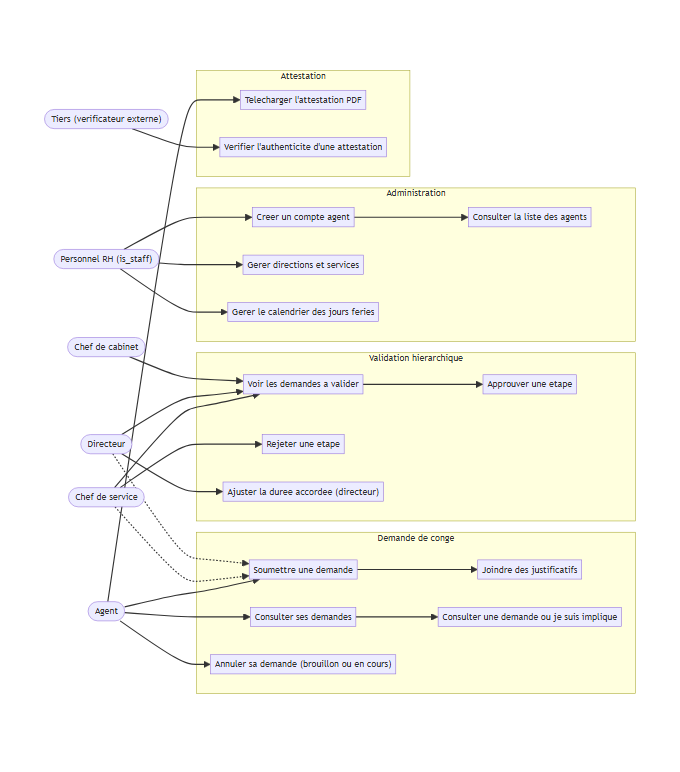
\includegraphics[width=0.95\textwidth]{images/diagrammes/01-cas-utilisation.png}
    \caption{Diagramme de cas d'utilisation}
    \label{fig:cas-utilisation}
\end{figure}

Le diagramme de cas d'utilisation (figure~\ref{fig:cas-utilisation}) distingue les actions accessibles à chaque rôle~: un agent soumet et suit ses propres demandes, un validateur (chef de service, directeur ou chef de cabinet) traite les demandes qui lui sont soumises, le personnel des ressources humaines gère les comptes et l'organisation, et toute personne extérieure peut vérifier l'authenticité d'une attestation sans se connecter.

\begin{figure}[htbp]
    \centering
    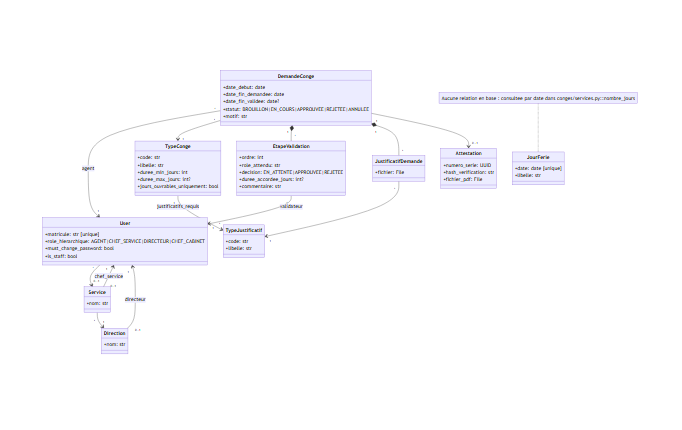
\includegraphics[width=0.95\textwidth]{images/diagrammes/02-classes.png}
    \caption{Diagramme de classes du modèle de données}
    \label{fig:classes}
\end{figure}

Le diagramme de classes (figure~\ref{fig:classes}) présente les entités du domaine et leurs relations. Le circuit de validation est modélisé par une séquence d'objets \texttt{EtapeValidation} liés à une \texttt{DemandeConge}, plutôt que par un simple champ de statut, afin de conserver la trace complète de chaque décision.

\begin{figure}[htbp]
    \centering
    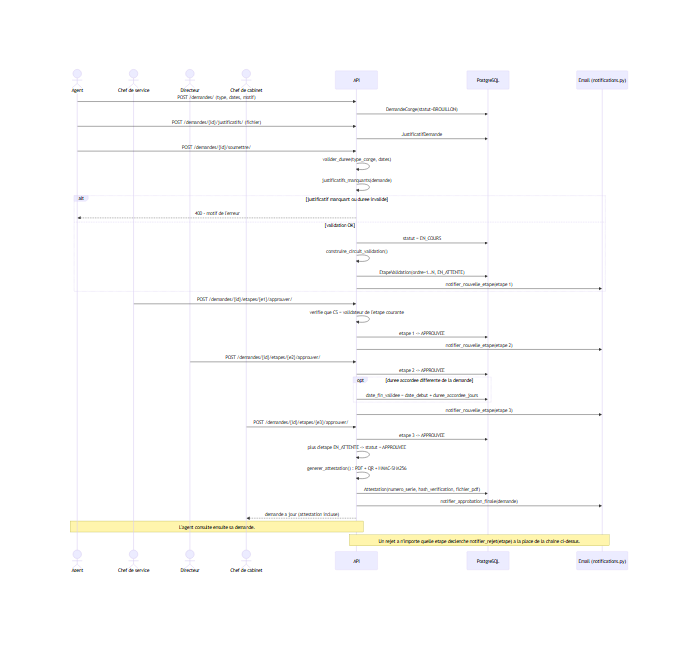
\includegraphics[width=0.85\textwidth]{images/diagrammes/03-sequence.png}
    \caption{Diagramme de séquence du parcours de validation}
    \label{fig:sequence}
\end{figure}

Le diagramme de séquence (figure~\ref{fig:sequence}) retrace le parcours complet d'une demande, de sa soumission jusqu'à la délivrance de l'attestation, avec les notifications envoyées à chaque changement de validateur.

\begin{figure}[htbp]
    \centering
    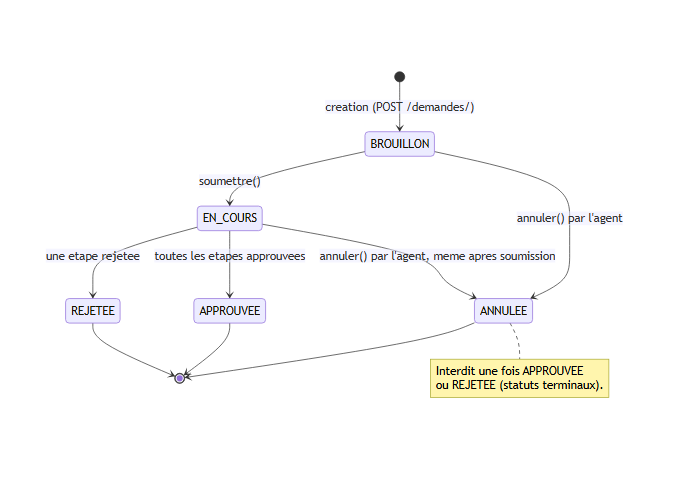
\includegraphics[width=0.7\textwidth]{images/diagrammes/04-etat-demande.png}
    \caption{Diagramme d'état d'une demande de congé}
    \label{fig:etat-demande}
\end{figure}

\begin{figure}[htbp]
    \centering
    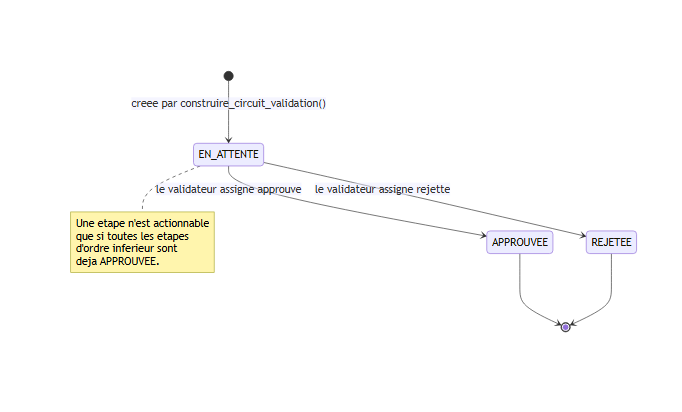
\includegraphics[width=0.7\textwidth]{images/diagrammes/05-etat-etape.png}
    \caption{Diagramme d'état d'une étape de validation}
    \label{fig:etat-etape}
\end{figure}

Les deux diagrammes d'état (figures~\ref{fig:etat-demande} et~\ref{fig:etat-etape}) précisent respectivement le cycle de vie complet d'une demande et celui d'une étape de validation prise isolément, notamment les conditions dans lesquelles une demande peut être annulée par son auteur.

\subsubsection{Développement de l'API et de la logique métier}

J'ai développé l'ensemble de l'API REST permettant la soumission d'une demande, le dépôt des pièces justificatives, la consultation des demandes en cours, ainsi que les actions d'approbation, de rejet et d'annulation. Chaque règle métier, comme le calcul du nombre de jours ouvrables ou la vérification des justificatifs requis, est validée côté serveur et non uniquement côté interface, afin de ne jamais faire reposer la fiabilité du système sur le seul navigateur de l'utilisateur.

\subsubsection{Authenticité des attestations}

J'ai conçu et développé le mécanisme de délivrance des attestations de congé. Chaque attestation approuvée est générée automatiquement au format PDF et porte un numéro de série ainsi qu'un code de vérification calculé par une fonction de hachage cryptographique, couplé à un code QR permettant une vérification publique en ligne, sans authentification préalable et sans exposer d'information sensible en cas de code incorrect.

\subsubsection{Développement de l'interface utilisateur}

J'ai développé l'ensemble des écrans de l'application~: connexion par matricule, dépôt d'une demande avec justificatifs dynamiques selon le type de congé choisi, suivi personnel des demandes, file d'attente des demandes à valider pour chaque niveau hiérarchique, et écrans d'administration permettant au personnel des ressources humaines de créer des comptes agents et de gérer la structure organisationnelle du ministère (directions et services).

\subsubsection{Sécurisation de l'application}

J'ai porté une attention particulière à la sécurité de l'application, celle-ci manipulant des données personnelles et parfois médicales. J'ai mis en place un contrôle d'accès strict à chaque niveau de l'API, une protection contre les tentatives répétées de connexion, un service de fichiers authentifié pour les justificatifs et les attestations, ainsi que les réglages nécessaires à un déploiement en HTTPS derrière un serveur mandataire inverse.

\subsubsection{Tests et fiabilisation}

J'ai systématiquement accompagné chaque fonctionnalité de tests automatisés, aussi bien côté serveur, pour vérifier la logique métier et les permissions, que dans un navigateur réel, pour vérifier le fonctionnement effectif de l'application du point de vue de l'utilisateur. Cette dernière catégorie de tests m'a permis de détecter et de corriger plusieurs anomalies avant qu'elles n'atteignent un environnement réel, notamment un problème de configuration lié à la protection contre les attaques CSRF entre l'interface et l'API.

\subsubsection{Conteneurisation et mise en production}

Enfin, j'ai mis en place une conteneurisation complète de l'application avec Docker, incluant un serveur mandataire inverse pour le chiffrement HTTPS et un mécanisme de sauvegarde automatisée de la base de données, ainsi qu'une chaîne d'intégration continue exécutant l'ensemble des tests à chaque modification du code.

\subsection{Difficultés rencontrées}

...

\subsection{Solutions apportées}

...

%%%%%%%%%%%%%%%%%%%%%%%%%%%%%%%%%%%%%%%%%%%%%%%%%%%%%%
% APPORTS DU STAGE
%%%%%%%%%%%%%%%%%%%%%%%%%%%%%%%%%%%%%%%%%%%%%%%%%%%%%%

\section{APPORTS DU STAGE}

\subsection{Compétences techniques}

Ce stage, réalisé au sein du service informatique du Ministère de l’Économie, des Finances et du Budget, m’a permis de m’intégrer dans un environnement professionnel structuré et de découvrir concrètement le fonctionnement d’un service informatique au sein d’une administration publique.

Cette expérience avait pour objectif de mettre en pratique les connaissances acquises au cours de ma formation et de développer mes compétences techniques dans différents domaines de l’informatique. Au cours de mon stage, j’ai notamment été amené à participer à la maintenance des équipements informatiques, à l’installation et à la configuration des postes de travail, ainsi qu’à l’assistance technique apportée aux différents utilisateurs du Ministère.

J’ai également eu l’occasion de renforcer mes connaissances dans le domaine des réseaux informatiques à travers différentes tâches liées à la connexion et à la configuration des équipements réseau. Ces activités m’ont permis de mieux comprendre l’importance de la disponibilité, de la fiabilité et de la sécurité des infrastructures informatiques dans le fonctionnement quotidien d’une administration.

Au-delà des compétences techniques, ce stage m’a permis de développer mon sens de l’organisation, ma rigueur, mon autonomie et ma capacité à analyser et résoudre des problèmes techniques. Les échanges avec les techniciens, les responsables du service et les différents utilisateurs m’ont également permis d’améliorer mes capacités de communication et de travail en équipe.

Ainsi, ce stage constitue une expérience professionnelle enrichissante qui m’a permis de mieux comprendre les réalités du métier d’informaticien et de mettre en relation les connaissances théoriques acquises durant ma formation avec des situations concrètes rencontrées dans le milieu professionnel.


\subsection{Compétences personnelles}

Ce stage au sein du service informatique du Ministère de l’Économie, des Finances et du Budget m’a permis de développer non seulement mes compétences techniques, mais également plusieurs qualités personnelles indispensables dans un environnement professionnel.

J’ai notamment développé mon sens de l’organisation et de la responsabilité en participant à différentes tâches informatiques tout en respectant les consignes et les procédures mises en place au sein du service. La diversité des interventions auxquelles j’ai été confronté m’a également permis d’améliorer ma capacité d’adaptation et de m’habituer à travailler sur différentes situations techniques.

Ce stage m’a aussi permis de renforcer ma rigueur et mon attention aux détails. En informatique, une simple erreur lors de la configuration d’un poste, d’un équipement réseau ou d’un périphérique peut entraîner des difficultés pour l’utilisateur. J’ai donc appris à effectuer mes tâches avec davantage de précision et à vérifier mon travail avant de le considérer comme terminé.

J’ai également développé mon autonomie et ma capacité à résoudre des problèmes. Face à une difficulté technique, j’ai appris à analyser la situation, à rechercher l’origine du problème et à proposer une solution adaptée, tout en sollicitant l’aide des techniciens lorsque cela était nécessaire.

Le travail au sein du service informatique m’a également permis d’améliorer mes capacités de communication et de travail en équipe. Les échanges avec les responsables, les techniciens et les différents utilisateurs m’ont appris à mieux écouter les besoins, à expliquer les problèmes techniques de manière simple et à collaborer efficacement avec les autres membres du service.

Enfin, cette expérience m’a permis de gagner en confiance et de mieux comprendre les exigences du monde professionnel. Elle a renforcé mon intérêt pour le domaine de l’informatique et m’a permis de développer des qualités telles que la ponctualité, la patience, la curiosité, l’esprit d’initiative et le sens des responsabilités.


%%%%%%%%%%%%%%%%%%%%%%%%%%%%%%%%%%%%%%%%%%%%%%%%%%%%%%
% CONCLUSION
%%%%%%%%%%%%%%%%%%%%%%%%%%%%%%%%%%%%%%%%%%%%%%%%%%%%%%

\section{CONCLUSION ET PERSPECTIVES}

\subsection{Bilan général}


Ce stage effectué au sein du service informatique du Ministère de l’Économie, des Finances et du Budget m’a permis de découvrir concrètement le fonctionnement d’un service informatique dans un environnement professionnel structuré et exigeant. Il m’a donné l’occasion de mettre en pratique les connaissances théoriques acquises au cours de ma formation et de développer de nouvelles compétences techniques à travers les différentes missions qui m’ont été confiées.

Au cours de cette expérience, j’ai notamment participé à des activités liées à l’installation et à la configuration des ordinateurs, à la connexion et à la configuration des périphériques, à la maintenance des équipements informatiques ainsi qu’à différentes interventions liées aux réseaux informatiques. Ces différentes tâches m’ont permis de mieux comprendre le fonctionnement des infrastructures informatiques et leur importance dans le bon déroulement des activités administratives du Ministère.

Au-delà des compétences techniques, ce stage m’a également permis de renforcer plusieurs qualités personnelles, notamment la rigueur, l’organisation, l’autonomie, le sens des responsabilités, la capacité d’adaptation et le travail en équipe. La réalisation de différentes tâches et la résolution de problèmes techniques m’ont appris à être plus méthodique, à analyser les situations avant d’intervenir et à respecter les procédures établies.

Les échanges avec les techniciens, les responsables du service et les différents utilisateurs m’ont également permis d’améliorer mes capacités de communication et de mieux comprendre les exigences du milieu professionnel. Cette expérience m’a ainsi permis de développer davantage ma confiance en moi et mon autonomie dans la réalisation des tâches qui m’étaient confiées.



En perspective, cette expérience constitue une base importante pour la poursuite de mon parcours académique et professionnel. Elle m’a permis de mieux comprendre les réalités du métier d’informaticien et de confirmer l’importance de développer continuellement mes connaissances dans le domaine des technologies de l’information.

Ce stage m’encourage notamment à approfondir mes compétences en réseaux informatiques, en administration des systèmes, en maintenance informatique et en sécurité des infrastructures. Je souhaite également continuer à développer mes connaissances dans les domaines liés à la cybersécurité et aux nouvelles technologies afin de mieux répondre aux besoins des organisations.

Ainsi, cette expérience professionnelle représente une étape importante dans mon parcours. Elle m’a permis de mieux identifier mes points forts, de prendre conscience des compétences que je dois encore améliorer et de me préparer progressivement à relever de futurs défis dans le domaine de l’ingénierie informatique.


%%%%%%%%%%%%%%%%%%%%%%%%%%%%%%%%%%%%%%%%%%%%%%%%%%%%%%
% ANNEXES
%%%%%%%%%%%%%%%%%%%%%%%%%%%%%%%%%%%%%%%%%%%%%%%%%%%%%%

\section*{ANNEXES}
\addcontentsline{toc}{section}{VII- ANNEXES}

...

\end{document}
